\section{Introduction}
\label{sec:introduction}
%\KZ{This para should talk about why you need slogan in e-commerce. You should
%picture a scenario from user point of view, not from system point of
%view.}
Traditionally, item-based recommendation~\cite{linden2003amazon,sarwar2001item} 
recommends too much products to users based on their historical behaviors.
\cut{
%Usually, the topic candidates are built from frequent phrases collected via 
%thoroughly analyzing query logs and product titles in order to cover as many user interests as possible.
%We leverage E-commerce knowledge base to constrain topics
%to a phrase which consists of a \emph{Category} 
%modified by a reasonable Property Value.
We first collect frequent phrases from 
query logs and product titles
in order to cover as many
user interests as possible.
Then, we construct topics from those phrases using E-commerce knowledge base.
%which makes it more reasonable and more convenient to organize items for topics.
The E-commerce knowledge base consists of three named 
entities:
%There are three named entity types in typical E-commerce knowledge base,
%there are three named entity types:
\emph{Category} (CG), \emph{Property Key} (PK) and \emph{Property Value} (PV). 
As shown in \figref{fig:cpv},
``Light fixture" is a Category, 
while ``Material" denotes a Property Key, which is the name of one product property.
``Glass"  and ``Plastic" are concrete property values of ``Material".
We constrain the topic to a phrase which consists of a Category modified by a reasonable Property Value.
Following this constraint, the topic can be associated with 
a set of items belong to the Category with the corresponding Property Value.
For example, ``glass light fixture" is a satisfied topic,
which the Category ``light fixture" is modified
by the concrete Property Value ``glass" of its 
corresponding product property ``Material".
Note that, ``Tools for baking" in \figref{fig:cpv}
also represents a topic which can be seen as the Category
``Tools for baking'' modified by an empty Property Value. 
 
\begin{figure}[th!]
	\centering
	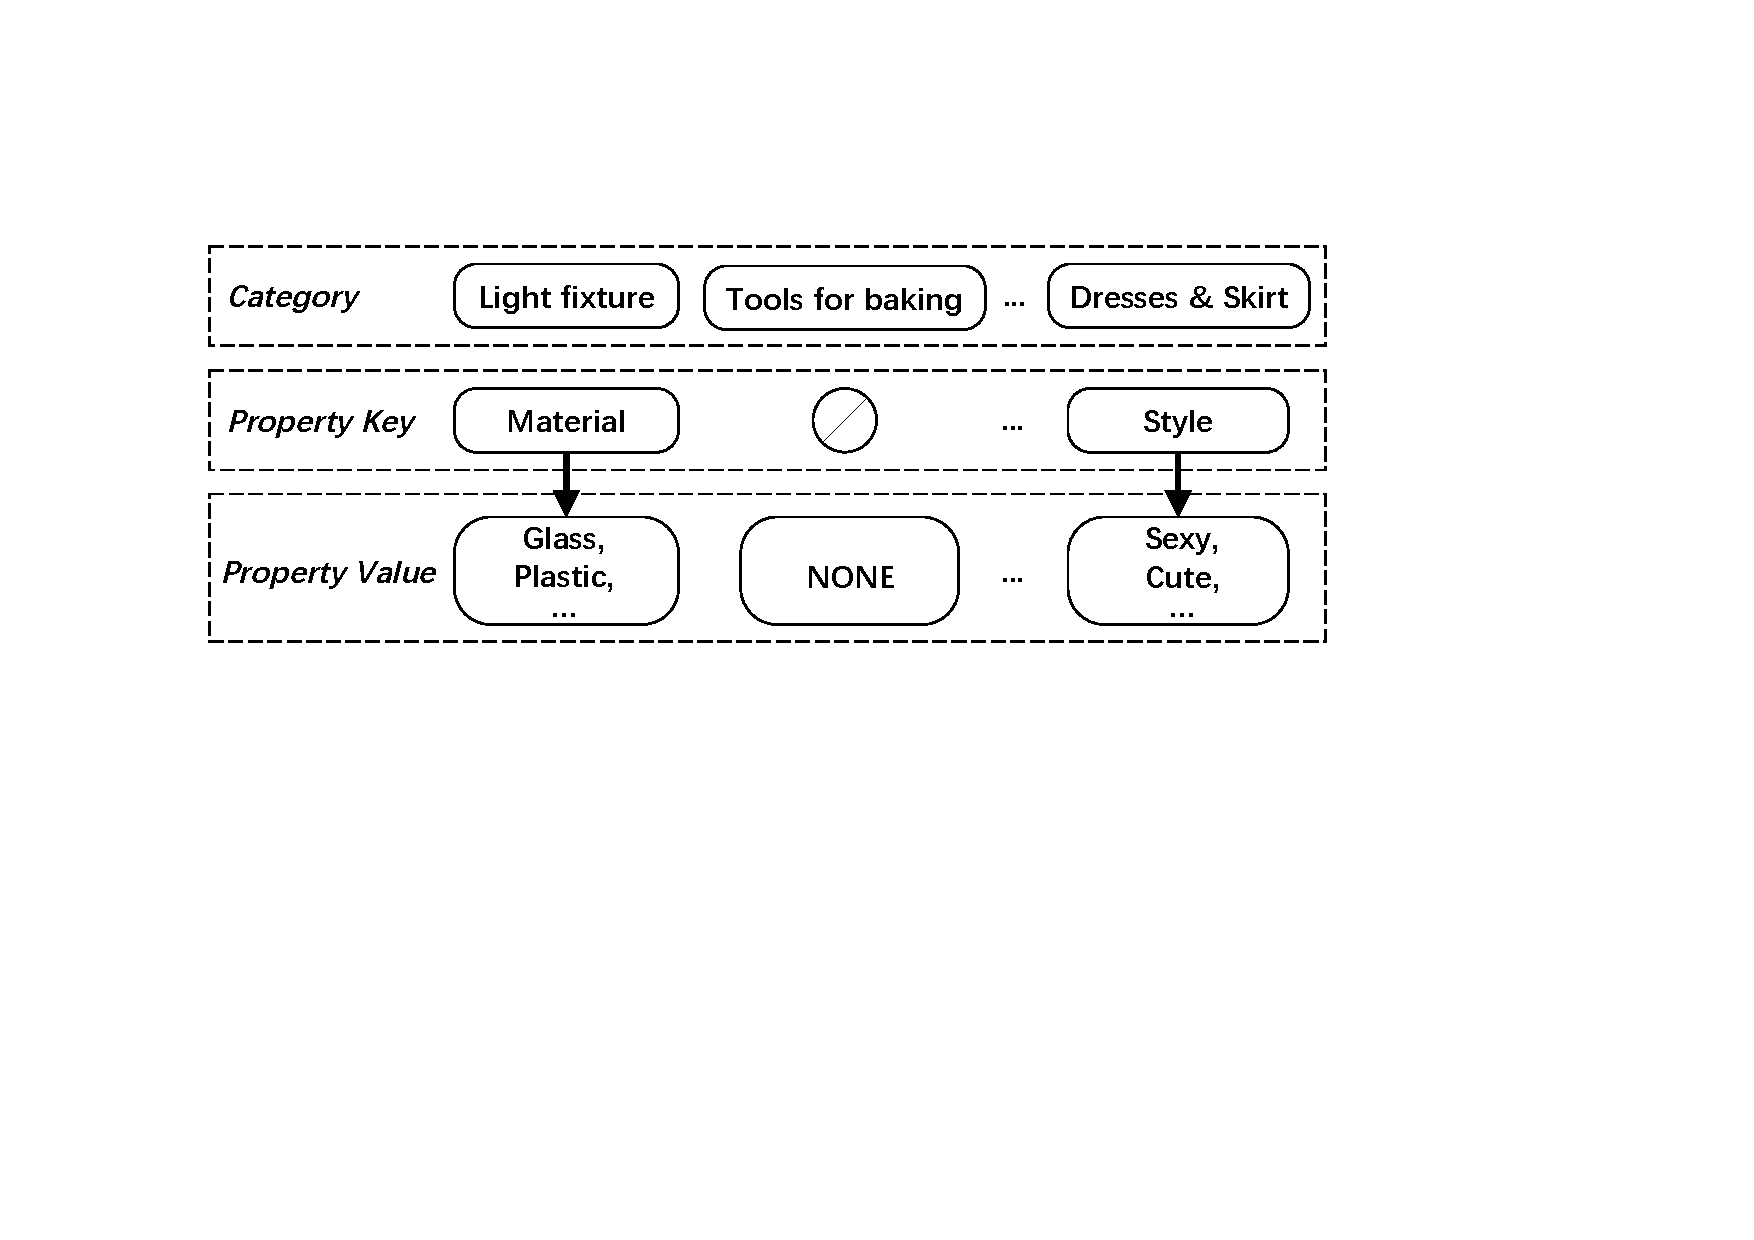
\includegraphics[width=0.95\columnwidth]{figures/cpv2}
	\caption{The structure of E-commerce knowledge-base.}
	\label{fig:cpv}
\end{figure}
}
Recently, topic-based recommendation~\cite{luo2019conceptualize} are proposed to conceptualize user needs as coarse-grained topics associating with items across fine-grained categories, which conducts the recommendation effectively and provides superior shopping experience to users. It is crucial to generate quality titles (called \emph{slogan}) for a coarse-grained topic against one particular aspect (called \emph{selling point}) each.
A informative and attractive slogan summarizes topic information and highlight selling point which promotes user's interests as well as help users make an informed decision and eventually improve shopping experience.
\figref{fig:example} demonstrates the topic-based recommendation scenario (left) with "glass light-fixture" topic across 
fine-grained categories such as ``beside lamp'' and ``ceiling light'' (middle) associating a number of items (left).
For a coarse-grained topic, each affiliated fine-grained category provides an aspect of the coarse-grained topic which can be used as a hint for the selling point exploration.
For example, \figref{fig:example} (right bottom) shows a number of items belong to \emph{bedside lamp} (category) enlighting \emph{bright and warm} as a selling point for customers.

%In the real implementation of recommendation, E-commerce platforms (such as Taobao~\footnote{http://www.taobao.com} App)
%usually combine item-based recommendation with topic-based recommendation.
%Among normal recommended items, the recommended topic is displayed to users as a card with its textual description and 
%the picture of a representative item (\figref{fig:example} left). 
%Taobao App incorporates the topic-based recommendation 
%into recommendation system to satisfy the scenario of coarse-grained recommendation.
%As shown in \figref{fig:topic} \textbf{PLACEHOLDER},
%the topic ``glass light fixture" is displayed to users as a card with
%its textual description and the picture of a representative item (left).
%Once a user clicks on it, he will enter into another page (right) where
%different items satisfied the needs of ``glass light fixture" are displayed.
%Such textual descriptions of topics are like salespeople,
%that is critical to demonstrate the recommended topics to customers.
%Quality textual descriptions attract users' attention, promote users' interests and eventually convince users to buy the recommended products.
%An informative and attractive textual description summarizes topic information and 
%highlights features of associated items which could help 
%users make an informed decision as well as promote users' interests and eventually improve the likelyhood of purchase.
%An informative and attractive textual description summarizes
%topic information and highlights \emph{selling points} of associated
%items which could promote users' interests as well as help users make an informed decision and eventually improve shopping experience.
%A selling point is supposed to highlight common property or function shared by items.
%For example, \emph{Boho style} (property) dresses, shoes and handbags make customer enjoying \emph{cool summer}.
%\figref{fig:example} (right bottom) shows a number of items belong to \emph{bedside lamp} (category or function) enlighting \emph{bright and warm} as a selling point for customers.
%For example, \figref{fig:boximiya} shows a number of items with common property Boho style enlighting \emph{cool summer} as a selling point for customers.
%Thus, the property or category usually need to be provided as a hint to craft quality slogans.

% 
%We suppose that items of  same fine-grained category shared common properties are 
%Items shared common properties are supposed to explore those selling points. Such selling points are explored from items shared common properties or use  Thus, a coarse-grained topic could be decomposed into various focuses referring to different selling points by its associated fine-grained categories.
%Given a topic, multiple slogans could be generated which highlight different features (or selling points) of associated items across 
%fine-grained categories. 
%However, until now, most of the textual descriptions for topics in the online shopping platforms
%namely \emph{slogan},
%are still created manually, 
%which is tedious, time-consuming, and less effective.

%On the other hand, such slogans should be personalized based on the item preferences
%which highlights the selling points to users
%and promotes their interests accordingly.

%We formulate it as a text-to-text generation problem.
%Specially, the system can intelligently generate quality slogans for a specific topic based on the given topic information and item preferences.

\begin{figure}[th!]
	%	\small
	\centering
	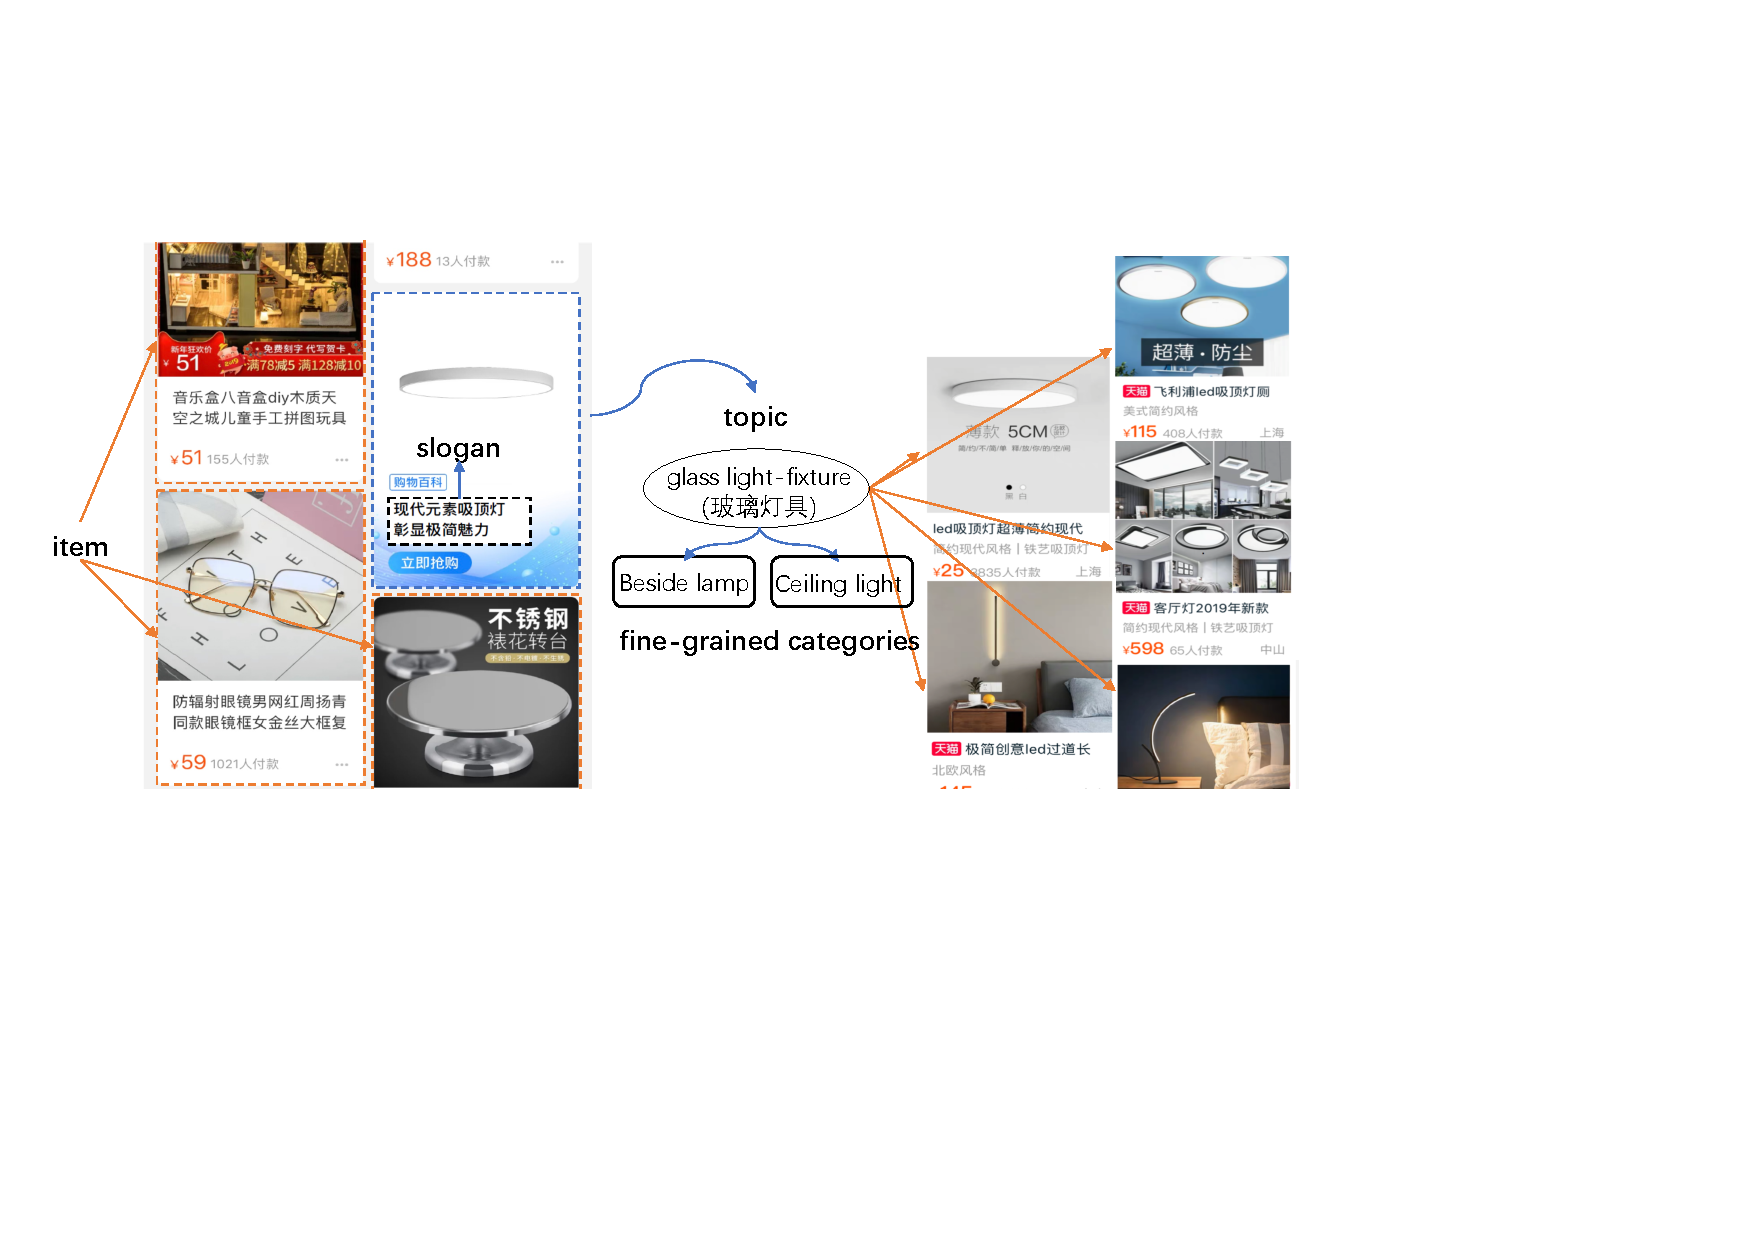
\includegraphics[width=0.95\columnwidth]{figures/example}
	\caption{An motivating example of slogan generation in E-commerce. }
\label{fig:example}
\end{figure}


Slogan generation in E-commerce is a relative new problem.
The most related works are product title generation~\cite{suzuki2011automatic,mathur2017generating,de2018generating}
and product description generation in E-commerce~\cite{langkilde1998generation,wang2017statistical}.
Existing works on product title generation are mostly 
selection-based and statistical-based.
Most prior works are based on templates and traditional statistical frameworks which are suffered from incoherence and lack of diversity,
thus are insufficient to generate quality titles or descriptions.
Recently, Chen et al.~\cite{ChenLZYZ019} extend the encoder-decoder framework to product description generation and achieve better performance. 

%We formulate personalized slogan generation as a text-to-text generation task.
%Owing to the tremendous success of
In this paper, we focus on automating the slogan generation
for online shopping in E-commerce.
%We suppose that slogans highlights features (or selling points) for the associated items of topics.
%Since items across categories are 
%in order to capture users' intentions and further promote user's interests.
%Each topic conceptualizes user interests and is associated with a bunch of items across 
%fine-grained categories and brands.
%quality slogans for topics are supposed to summarize topics' information and expose features or selling points of associated items.
%One of the biggest challenges is to explore features 
%for the associated items of topics and express 
%those features as specific selling points in generated slogans to further extend the user interests implied by the topic.
Crafting a successful slogan for specific topic is tedious and highly time-consuming.
Besides, previous related works are mainly use templates or statistical methods which are insufficient to achieve satisfying performance.
Recently, convolutional sequence-to-sequence (Seq2Seq) learning has been achieved tremendous success in many text generation applications.
Owing to this success, 
we extend the effective convolutional Seq2Seq framework~\cite{ott2019fairseq}
and propose a 
\textbf{S}emantics-enhanced \textbf{S}logan \textbf{G}eneration (or SSG) 
model to automatically generate quality slogans for 
online topic-based recommendation.
SSG introduces \emph{item preferences} based on fine-grained categories
to provide more information which specifies
various aspects of topics, then
incorporates \emph{is-a} knowledge for better contextualized representations
and eventally generates more accurate and attractive slogans.
To provide a dataset for the automatic slogan generation,
we construct and make publicly available a new dataset from Taobao.
We collect 857 topics and in total 3,555 pairs of topic and provided with an aspect hint (i.e. fine-grained category)
and manually created slogan accordingly.
We also retrieve the \emph{is-a} knowledge
from a external knowledge base in Chinese.
The involved \emph{is-a} knowledge will be released together with previous created dataset.
The contributions of this paper are summarized below:
\begin{itemize}
	\item We define a new problem slogan generation, 
	generating accurate and attractive slogans,which benefits existing
	recommendation systems in E-commerce.
	\item We propose a novel model SALE based-on sequence-to-sequence learning, 
	which utilizes item preferences and further incorporates the hypernym-hyponym semantic knowledge to improve the quality of generation. Extensive experiments show that our approach outperforms several baselines by a substantial margin.
	\item We create a new dataset for automatic slogan generation (\secref{sec:eval_dataset}).
	We intend to release this dataset as well as the implementation of the proposed method for future work in this research area. 
\end{itemize}


%we build various preferred item sets for topics to represent users' preferences accordingly
%by introducing category ontology in E-commerce.
%Such item sets reflect different focuses and potential interests of users.

%讲一下personalize
%users needs - topic - items
%user preferences - secondary category - items


%The most related work are about product description generation and 
%title generation for browse pages.
%
%We introduce the category ontology 
%In topic-based recommendation, a topic bridges user needs and its associated items.
%Similarly, user preferences to a specific topic can be expressed by  
%Similarly, category ontology is introduced as potential focuses
%connecting user preference and items.





%It is necessary to make the slogan focuses adapted to 
%the selling points conducting by users' preferences of items.
%
%A set of associated items represents the users' needs
%by summarizing and con
%A set of preferred items which relevant to a specific topic
%can represent the users' preferences 
%It is reasonable to represent the users' preferences
%of a specific topic as a set of preferred items
%which are relevant to the topic. 
%Besides, such item preferences 
%Different from exploring users' preference from private information,
%we represent the preferences as a set of preferred items relevant to
%a specific topic.
%The system is expzected to explore selling points from 
%the topic and the provided preferred items,

%\begin{figure}[th!]
%	\centering
%	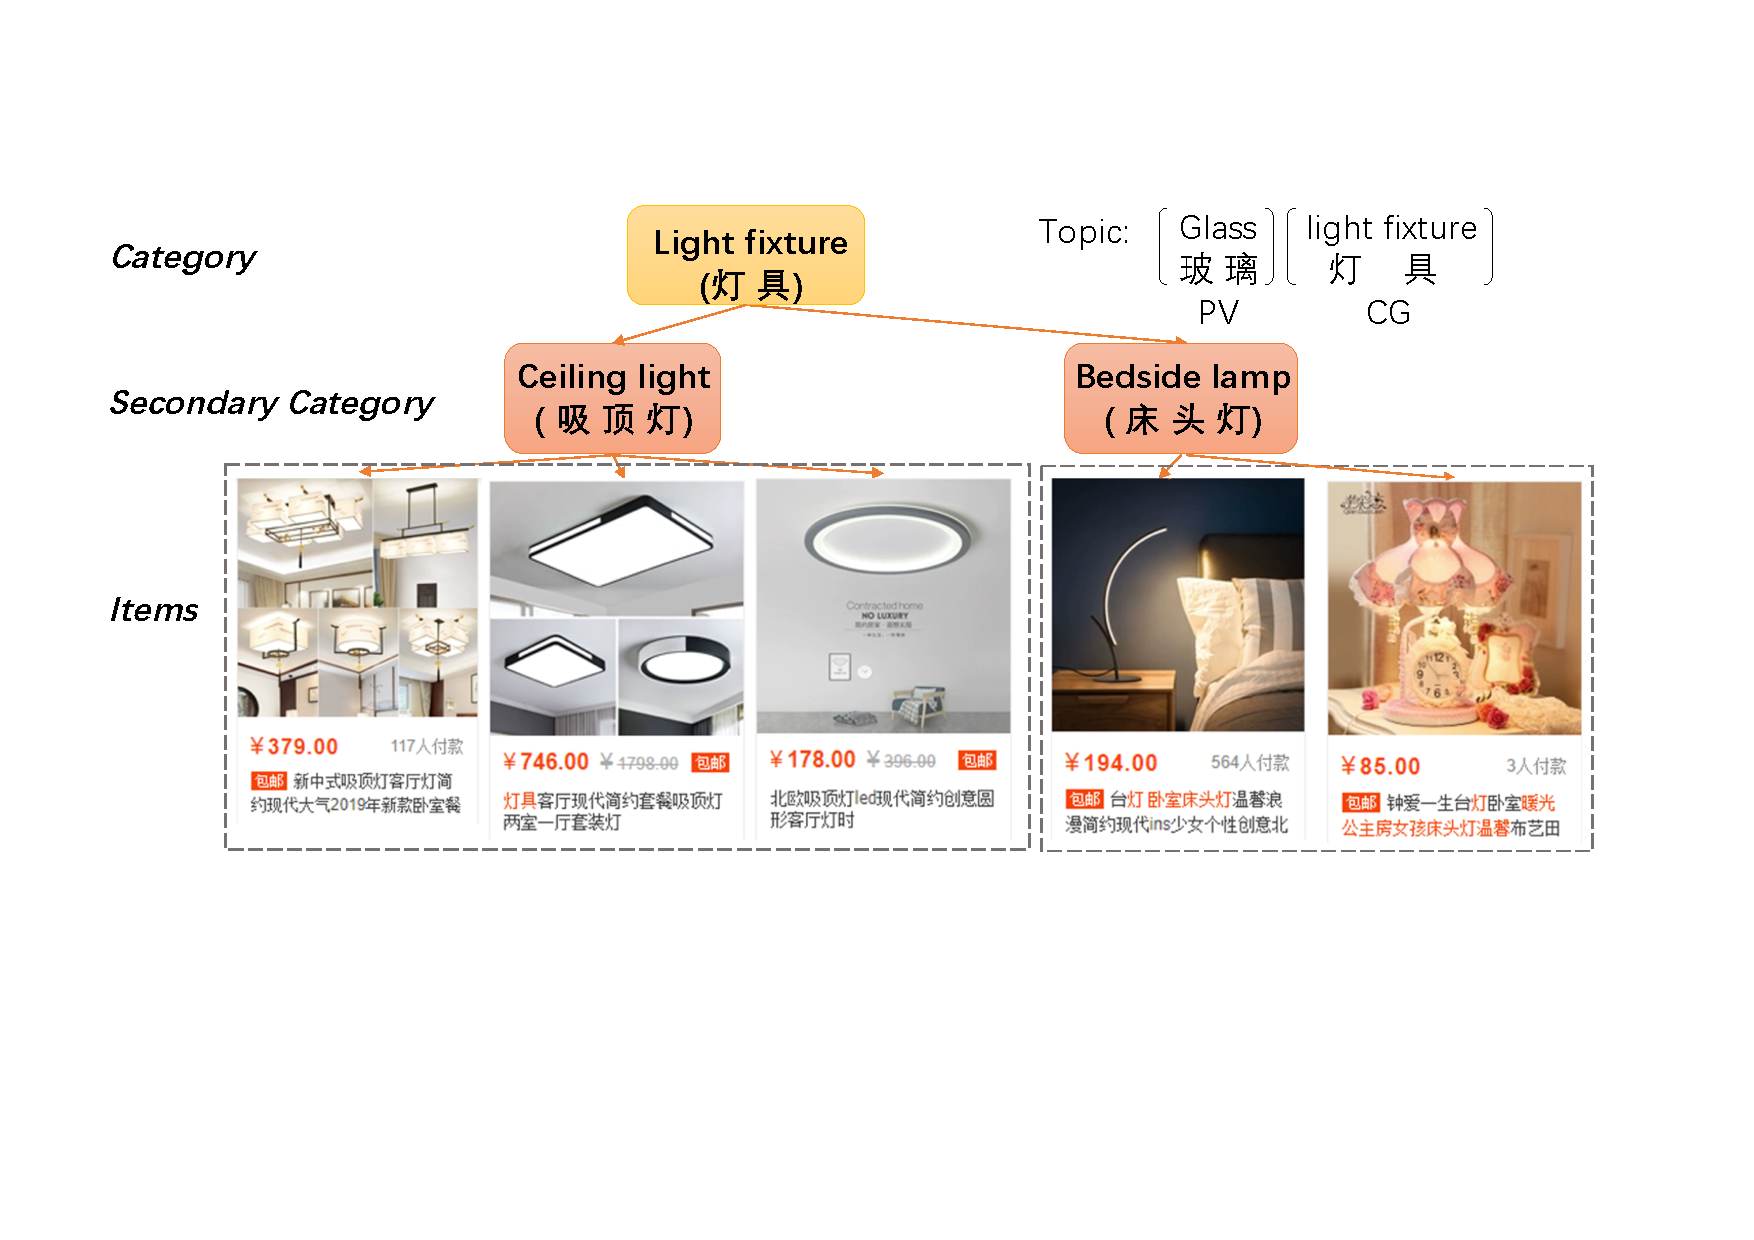
\includegraphics[width=0.95\columnwidth]{figures/cate8}
%	\caption{An example of category structure in E-commerce.}
%	\label{fig:cate}
%\end{figure}




%One of the biggest challenges of recommendation in E-commerce is to 
%efficiently  in an accurate and attractive way.


%说为topic生成标题的重要性

%item-specific details
%attract customer's attention and transfer it to purchase
%别人是怎么做的 局限性在哪


%In this paper, 
%我们要做的是啥
%说明下我们的topic是啥
%我们准备怎么做

%最后总结一下我们的贡献是啥

%related work
%item-based recommendation 展示: product description generation
%topic-based recommendation 展示: slogan generation

%E-commerce platforms traditionally present and recommend items to users using titles and demo pictures from on-line merchants that describe items information.  
% limitations

%To resolve these limitations, instead of \emph{item-based} presentation and recommendation, recent works focus on exploring user needs and propose \emph{topic-based} presentation and recommendation~\cite{}.



%[ebay emnlp 2018] Generating E-Commerce Product Titles and Predicting their Quality
%[kdd 2019] Towards Knowledge-Based Personalized Product Description Generation in E-commerce
%[ICML 2019] Generative Adversarial User Model for Reinforcement Learning Based Recommendation System
